\documentclass{article}
\usepackage[utf8]{inputenc}

\title{Redes Neurais no CIn UFPE}
\author{João Vitor Alves Almeida }
\date{October 2019}

\usepackage{natbib}
\usepackage{graphicx}

\begin{document}

\maketitle

\section{Introdução}
A disciplina eletiva de Redes Neurais(if702)\citep{Disciplina} do Centro de Informática da UFPE é oferecida pelo professor Germano Vasconcelos\citep{GCV}, ao segundo semestre de cada ano. A disciplina explora vários conceitos e abordagens das redes neurais —estruturas com capacidade de aprendizagem, que promovem a classificação de dados, após o devido treinamento. A disciplina é dividida em 4 partes, sendo elas os Fundamentos básicos ("Introdução e fundamentos matemáticos" e "Fundamentos e modelos de aprendizagem"), Arquiteturas e Modelos Redes feedforward("Adaline e Perceptrons", "Multilayer Perceptrons (MLP)", "Redes de Funções de Base Radial (RBF)" e "Máquina de Vetores de Suporte (SVM)"), Redes recorrentes("Rede de Jordan e Elman") e Redes auto-organizáveis("De Hopfield", "De Kohonen" e "ART")\citep{CInWiki}. \\

\begin{figure}[h!]
\centering
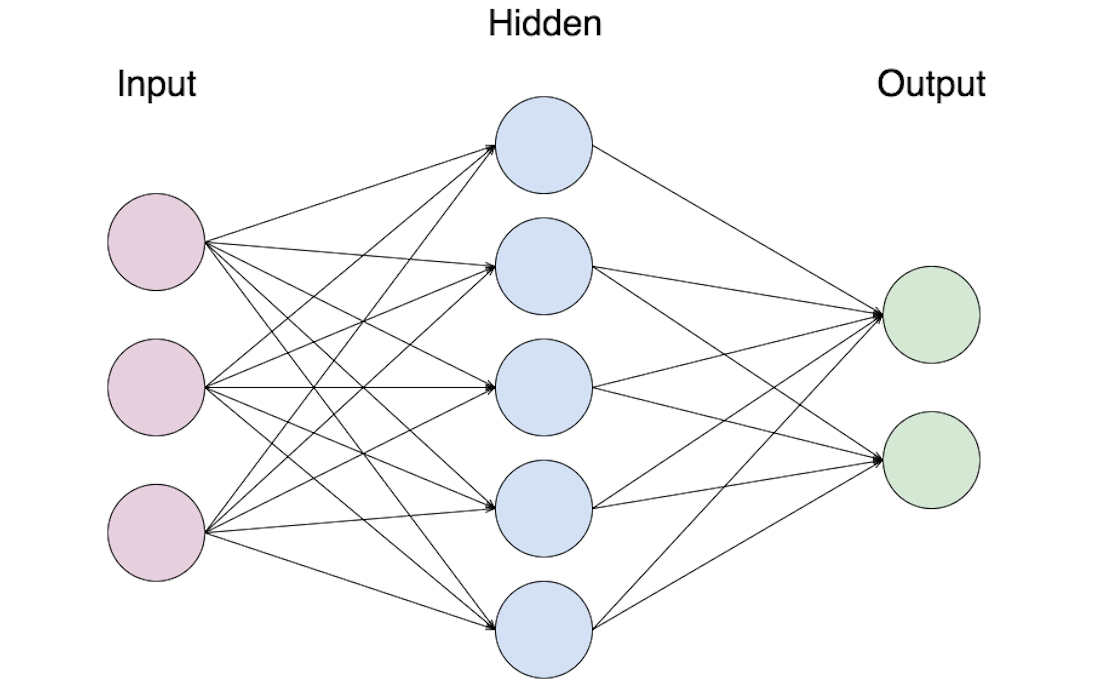
\includegraphics[scale=0.2]{redes-1.png}
\caption{Redes Neurais}
\label{fig:redes-1}
\citep{RedesNeurais}
\end{figure}



{
A Disciplina de Redes Neurais faz parte da grande área da computação chamada de aprendizagem de máquina. Uma área relativamente recente que trabalha com sistemas inteligentes que, diferentemente dos algoritmos usuais, funcionam na base do treinamento repetitivo prévio.    
}



\section{Relevância}
O Universo das inteligencias artificiais está em rápido crescimento
devido a sua extensa gama de atuação. O conhecimento que a disciplina de redes neurais têm a oferecer possibilita uma boa base para o completo entendimento da aprendizagem de máquina.


\begin{figure}[h!]
\centering

\includegraphics[scale=0.1]{redesneurais.jpg}
\caption{Redes Neurais}
\label{fig:redesneurais}
\citep{RedesNeurais2}
\end{figure}


\section{Relação com outras Disciplinas}
A disciplina de redes neurais tem uma forte relação com todas as cadeiras da categoria de Sistemas Inteligentes dos componentes eletivos do CIn, sendo elas: IF703-AGENTES AUTONOMOS ELETIVO
/ IF699-APRENDIZAGEM DE MAQUINA ELETIVO / IF705-AUTOMACAO INTELIGENTE ELETIVO / IF701-ENG.CONHEC.SISTEMAS ESPECIALISTAS ELETIVO / IF797-OTIMI- ZACAO ELETIVO / IF700-PERCEP. COMPUTAC.E RECONH. PADRAO ELETIVO / IF704-PROCESSAMENTO LINGUAGEM NATURAL ELETIVO / IF702-REDES NEURAIS ELETIVO / IF707-SEMIN. EM INTELIGENCIA ARTIFICIAL ELETIVO / IF706-TOPICOS AVANC.INTELEG.ARTIFICIAL ELETIVO. Contudo, as aprendizagens da disciplina de Redes Neurais são aplicá- veis em qualquer área do conhecimento, tendo em vista que as IAs são muito resilientes.


\bibliographystyle{plain}
\bibliography{jvaa}
\end{document}
